%%%%%%%%%%%%%%%%%%%%%%%%%%%%%%%%%%%%%%%%%%%%%%%%%%%%%%%%%%%%%%%%%%%%%
%% This is a (brief) model paper using the achemso class
%% The document class accepts keyval options, which should include
%% the target journal and optionally the manuscript type. 
%%%%%%%%%%%%%%%%%%%%%%%%%%%%%%%%%%%%%%%%%%%%%%%%%%%%%%%%%%%%%%%%%%%%%
\documentclass[journal=jacsat,manuscript=article]{achemso}

%%%%%%%%%%%%%%%%%%%%%%%%%%%%%%%%%%%%%%%%%%%%%%%%%%%%%%%%%%%%%%%%%%%%%
%% Place any additional packages needed here.  Only include packages
%% which are essential, to avoid problems later. Do NOT use any
%% packages which require e-TeX (for example etoolbox): the e-TeX
%% extensions are not currently available on the ACS conversion
%% servers.
%%%%%%%%%%%%%%%%%%%%%%%%%%%%%%%%%%%%%%%%%%%%%%%%%%%%%%%%%%%%%%%%%%%%%
\usepackage[version=3]{mhchem} % Formula subscripts using \ce{}
\usepackage{todonotes}
\mciteErrorOnUnknownfalse
\usepackage{babel}
\setlength{\marginparwidth}{2cm}
\usepackage{xcolor}
%%%%%%%%%%%%%%%%%%%%%%%%%%%%%%%%%%%%%%%%%%%%%%%%%%%%%%%%%%%%%%%%%%%%%
%% If issues arise when submitting your manuscript, you may want to
%% un-comment the next line.  This provides information on the
%% version of every file you have used.
%%%%%%%%%%%%%%%%%%%%%%%%%%%%%%%%%%%%%%%%%%%%%%%%%%%%%%%%%%%%%%%%%%%%%
%%\listfiles

%%%%%%%%%%%%%%%%%%%%%%%%%%%%%%%%%%%%%%%%%%%%%%%%%%%%%%%%%%%%%%%%%%%%%
%% Place any additional macros here.  Please use \newcommand* where
%% possible, and avoid layout-changing macros (which are not used
%% when typesetting).
%%%%%%%%%%%%%%%%%%%%%%%%%%%%%%%%%%%%%%%%%%%%%%%%%%%%%%%%%%%%%%%%%%%%%
\newcommand*\mycommand[1]{\texttt{\emph{#1}}}

%%%%%%%%%%%%%%%%%%%%%%%%%%%%%%%%%%%%%%%%%%%%%%%%%%%%%%%%%%%%%%%%%%%%%
%% Meta-data block
%% ---------------
%% Each author should be given as a separate \author command.
%%
%% Corresponding authors should have an e-mail given after the author
%% name as an \email command. Phone and fax numbers can be given
%% using \phone and \fax, respectively; this information is optional.
%%
%% The affiliation of authors is given after the authors; each
%% \affiliation command applies to all preceding authors not already
%% assigned an affiliation.
%%
%% The affiliation takes an option argument for the short name.  This
%% will typically be something like "University of Somewhere".
%%
%% The \altaffiliation macro should be used for new address, etc.
%% On the other hand, \alsoaffiliation is used on a per author basis
%% when authors are associated with multiple institutions.
%%%%%%%%%%%%%%%%%%%%%%%%%%%%%%%%%%%%%%%%%%%%%%%%%%%%%%%%%%%%%%%%%%%%%
\author{Puthiyapurayil Sibeesh and T K Shajahan}
%\altaffiliation{A shared footnote}
%\author{T. K. Shajahan}
\email{shajahan@nitk.edu.in}
\phone{+123 (0)123 4445556}
\fax{+123 (0)123 4445557}
\affiliation[Unknown University]
{Department of Physics, National Institute of Technology Karnataka, India-575025}


%%%%%%%%%%%%%%%%%%%%%%%%%%%%%%%%%%%%%%%%%%%%%%%%%%%%%%%%%%%%%%%%%%%%%
%% The document title should be given as usual. Some journals require
%% a running title from the author: this should be supplied as an
%% optional argument to \title.
%%%%%%%%%%%%%%%%%%%%%%%%%%%%%%%%%%%%%%%%%%%%%%%%%%%%%%%%%%%%%%%%%%%%%
\title[An \textsf{achemso} demo]
  {Image acquisition and Electric field application in the BZ reaction by virtual instrumentation using LabVIEW\footnote{A footnote for the title}}

%%%%%%%%%%%%%%%%%%%%%%%%%%%%%%%%%%%%%%%%%%%%%%%%%%%%%%%%%%%%%%%%%%%%%
%% Some journals require a list of abbreviations or keywords to be
%% supplied. These should be set up here, and will be printed after
%% the title and author information, if needed.
%%%%%%%%%%%%%%%%%%%%%%%%%%%%%%%%%%%%%%%%%%%%%%%%%%%%%%%%%%%%%%%%%%%%%
\abbreviations{IR,NMR,UV}
\keywords{American Chemical Society, \LaTeX}

%%%%%%%%%%%%%%%%%%%%%%%%%%%%%%%%%%%%%%%%%%%%%%%%%%%%%%%%%%%%%%%%%%%%%
%% The manuscript does not need to include \maketitle, which is
%% executed automatically.
%%%%%%%%%%%%%%%%%%%%%%%%%%%%%%%%%%%%%%%%%%%%%%%%%%%%%%%%%%%%%%%%%%%%%
\begin{document}

%%%%%%%%%%%%%%%%%%%%%%%%%%%%%%%%%%%%%%%%%%%%%%%%%%%%%%%%%%%%%%%%%%%%%
%% The "tocentry" environment can be used to create an entry for the
%% graphical table of contents. It is given here as some journals
%% require that it is printed as part of the abstract page. It will
%% be automatically moved as appropriate.
%%%%%%%%%%%%%%%%%%%%%%%%%%%%%%%%%%%%%%%%%%%%%%%%%%%%%%%%%%%%%%%%%%%%%
\begin{tocentry}

Some journals require a graphical entry for the Table of Contents.
This should be laid out ``print ready'' so that the sizing of the
text is correct.

Inside the \texttt{tocentry} environment, the font used is Helvetica
8\,pt, as required by \emph{Journal of the American Chemical
Society}.

The surrounding frame is 9\,cm by 3.5\,cm, which is the maximum
permitted for  \emph{Journal of the American Chemical Society}
graphical table of content entries. The box will not resize if the
content is too big: instead it will overflow the edge of the box.

This box and the associated title will always be printed on a
separate page at the end of the document.

\end{tocentry}

%%%%%%%%%%%%%%%%%%%%%%%%%%%%%%%%%%%%%%%%%%%%%%%%%%%%%%%%%%%%%%%%%%%%%
%% The abstract environment will automatically gobble the contents
%% if an abstract is not used by the target journal.
%%%%%%%%%%%%%%%%%%%%%%%%%%%%%%%%%%%%%%%%%%%%%%%%%%%%%%%%%%%%%%%%%%%%%
\begin{abstract}
%This study is related to the instrumentation part of the experiments in Belousov-Zhabotinsky (BZ) reaction. 
We report simultaneous recording and delivering electrical stimuli
during the image acquisition of the experiments in the Belousov-Zhabotinsky (BZ) reaction. The excitation wave formation,
pinning, and unpinning in the BZ reaction is an important topic in the
field of nonlinear dynamics because of its similarity and scope of
applicability in biological systems. Unpinning studies in the BZ
reaction use low-voltage DC and AC electric fields. We explored
virtual instrumentation using LabVIEW and developed programs for both
DC and Polarised electric fields. Our programs simultaneously generate
the required voltage signals, capture and save the images for further
analysis.  We were able to collect the data with these codes and study
the mechanism of unpinning with DC and circularly polarised electric
field (CPEF).
\end{abstract}

%%%%%%%%%%%%%%%%%%%%%%%%%%%%%%%%%%%%%%%%%%%%%%%%%%%%%%%%%%%%%%%%%%%%%
%% Start the main part of the manuscript here.
%%%%%%%%%%%%%%%%%%%%%%%%%%%%%%%%%%%%%%%%%%%%%%%%%%%%%%%%%%%%%%%%%%%%%
\section{Introduction}
The Belousov-Zhabotinsky (BZ) reaction is a chemical reaction that
exhibits oscillating behavior and complex spatial patterns such as
target, spiral, and scroll waves. These types of waves can be found in
various systems, such as the aggregation of Dictyostelium discoideum
amoeba \cite{tan2020topological}, the chicken retina
\cite{yu2012reentrant}, the human brain \cite{rostami2018defects}, the
heart tissue \cite{lebert2023reconstruction}, and the reaction of CO
on platinum surfaces \cite{bhattacharya2019controlling}.  Collectively
referred to as excitable media, these systems have a similar
reaction to an exciting stimulus when it exceeds a certain threshold,
and then they do not respond to any additional stimulus for a specific
duration of time. The BZ reaction has been studied extensively in chemical kinetics and
nonlinear dynamics. The BZ reaction has been found to have several
interesting applications in biological systems, chemical computing
\cite{steinbock1996chemical}\cite{gruenert2013multi}, and
self-propelled motion
\cite{kumar2021fast}\cite{suematsu2018evolution}.
%%%%%%%%%%%%%%%%%%%%%%%%%%%%%%%%%%%%%%%%%%%%%%%%%%%%%%%%%%%%%%%%%%%%%%%%%%%%%%%%%%%%%%%%%%%%%%%%%%%%%%%%%%%%%%%%%%%%%%%%%%%%%%%%%%%%%%%%%%%%%%%%%%%%%%%%%
However, imaging the BZ reaction is challenging due to several
factors. The BZ reaction is a non-equilibrium process, and its
dynamics change with time. As a result, imaging the reaction requires
techniques to capture fast changes and non-stationary behavior. Hence
we trigger the camera with counter-output pulses, and the frequency of
the counter signal becomes the frame rate of the camera. The patterns
produced by the BZ reaction are difficult to detect because the
reaction occurs in a semi-transparent solution. We solved this problem
by illuminating a diffused white LED light source below the reaction
medium. Patterns observed in the BZ reaction are blue, so the
camera is mounted with a blue dichroic filter to enhance the
imaging. The patterns produced by the BZ reaction can be small and
require high spatial-resolution imaging techniques to
observe. Achieving sufficient resolution can be difficult, mainly if
the patterns are small or occur in a three-dimensional space. We use a
CCD camera with a maximum resolution of 640x480, and a user can choose
the resolution according to their requirement.  The BZ reaction is
sensitive to changes in temperature, and imaging the reaction requires
precise temperature control to ensure consistent behavior. Hence,
experiments were performed in an AC room with an ambient temperature.
%%%%%%%%%%%%%%%%%%%%%%%%%%%%%%%%%%%%%%%%%%%%%%%%%%%%%%%%%%%%%%%%%%%%%%%%%%%%%%%%%%%%%%%%%%%%%%%%%%%%%%%%%%%%%%%%%%%%%%%%%%%%%%%%%%%%%%%%%%%%%%%%%%%%%%%%%%%%%%%%%%%%%%%%
%%%%%%%%%%%%%%%%%%%%%%%%%%%%%%%%%%%%%%%%%%
Spiral or scroll waves can be anchored to inhomogeneities in the
medium and become more stabilized patterns. These pinned patterns play
a crucial role in the development of dynamic disorders, including
abnormal heart rhythms \cite{bruser2012automatic}
\cite{kundu2021amplitude} and epilepsy \cite{punacha2020theory}. The
BZ reaction can also be influenced by the application of an electric
field. When a low-voltage electric field is applied to the BZ
reaction, it can change the reaction rate and move the patterns that
are formed. This is because the electric field can alter the movement
of ions and electrons in the solution, affecting the kinetics of the
chemical reactions. Hence, applying a low-voltage electric field can
unpin the pinned waves from the inhomogeneities. Few experiments
reported the unpinning of the pinned waves using electric field
\cite{steinbock1992electric}\cite{ji2013experimental}\cite{jimenez2013electric}\cite{sutthiopad2014unpinning}\cite{porjai2016electrically},
and in those studies, the applied field is directly controlled using
constant current sources and programmable power supplies. The
experimental system requires multiple devices to function together.
Virtual instrumentation can effectively control such tasks. Virtual
instrumentation refers to the use of software and computer technology
to create and control virtual versions of physical instruments. These
virtual instruments can be used for various purposes, such as
scientific research, engineering design, and industrial automation.
Virtual instrumentation is a growing field and is increasingly used in
various industries, including telecommunications, aerospace, and
manufacturing.

LabVIEW (Laboratory Virtual Instrument Engineering Workbench) is a
graphical programming platform widely used for virtual
instrumentation. It allows users to create virtual instruments, also
known as virtual measurement systems, using a drag-and-drop interface
and a vast library of pre-built functions and tools. LabVIEW enables
users to acquire, analyze, and present data in a user-friendly and
customizable way. It also allows the integration of various hardware
devices and instruments, such as oscilloscopes, data acquisition
systems, and control systems, into a single system. A LabVIEW program
consists of a front panel and a block diagram. The front panel and
block diagram work together to create a complete program. The front
panel is the user interface of the LabVIEW program and serves as the
control center for the user. It consists of graphical objects such as
buttons, dials, sliders, and graphs that the user interacts with to
control the program and view the results. The block diagram is the
programming logic of the LabVIEW program and contains graphical
representations of the functions and operations performed by the
program. The block diagram consists of blocks, which are connected to
each other with wires that represent the flow of data. Each block
represents a specific operation, such as mathematical calculations,
data acquisition, or signal processing.

We developed a LabVIEW based virtual interface that can generate
voltage signals and capture the images of the patterns at the same
time by using LabVIEW software.  We use a multi-functional data
acquisition device (NI USB DAQ 6343) to create voltage signals and to
trigger a Charge Coupled Device (CCD) camera simultaneously. With our
virtual interface, a user can select the camera, trigger parameters,
amplitude, and frequency of the voltage signals with some mouse
clicks. In the BZ experiments, we need to observe the spiral waves
without an electric field and with an electric field. So, we developed
two scripts to capture the images before and after the field
generation. Later, we combined those two scrips and made them run
sequentially. We are able to make DC and polarised fields with two
different codes.  There are other reported works that use image
acquisition and electric field application. \cite{oddy2004method} Oddy
et al. and colleagues have created a technique based on LabVIEW for
measuring the electrophoretic mobility of fluorescently labeled
particles that are submicrometer in size, as well as the
electroosmotic mobility of a microchannel. They have established
explicit expressions for the unknown electrophoretic and
electroosmotic mobilities using particle displacements caused by
applied direct current (DC) and alternating current (AC) electric
fields. They capture images of the particle displacements using an
epifluorescent microscope and a CCD camera.  The standard technique to
terminate ventricular fibrillation (VF) is the high voltage direct
current (DC) shock, but it has the potential to cause significant pain
and tissue damage. The specific effect of the DC electric field on
depolarizing the heart during VF remains
uncertain. \cite{musunuri2009ventricular} Musunuri et al. postulated
and found that combining pacing with a low-energy DC field (pacing+DC)
could stop VF by altering the ventricular propagation pattern. They
conducted experiments on six Langendorff-perfusion isolated rabbit
hearts with the ablated sinoatrial (SA) node. The DC field was
administered to the left ventricle (cathode) and right ventricle
(anode). They developed a timed protocol utilizing LabVIEW programming
that delivers pacing, DC, and pacing+DC stimuli in two-second
intervals.  The precise and dynamic measurement of pupil size is
extremely valuable in researching various neuronal functions and
dysfunctions. Despite significant progress in image processing
techniques for determining pupil parameters, there has been relatively
little exploration of practical hardware concerns related to creating
image acquisition systems for pupil analysis. In their work, JKS De
Souza et al. \cite{ji2013experimental} and colleagues in 2013
presented and confirmed the key features of such a system, which is
based on a compact, commercially available, and inexpensive FireWire
digital camera. They successfully implemented two modes of video
recording, namely a continuous mode and an event-triggered mode. The
entire system's interoperability is ensured through a collection of
modular software components hosted on a personal computer and coded in
Labview.  Reddy, B et al. \cite{reddy2015development} has developed a
data acquisition unit for a Compact Airglow photometer (CAP) for
terrestrial and planetary emissions using LabVIEW Software. The data
acquisition unit interfaces a CCD camera with any personal computer.
Hence, our work has wide applications for low-energy electric field
experiments as well as image acquisition.
\section{Methods and Instrumentation}
\subsection{Experimental methods}
To monitor the motions of chemical waves, the experimental system is
illuminated with a diffused white light (Flat LED source) from below,
and the transmitted light is detected with a CCD camera
(mvBLUECOUGAR-X120bc). A tripod (Vanguard Espod CX 203AGH) is used as
a camera stand. The camera is mounted with a blue dichroic filter
(BP470-27) to increase the contrast between the pattern and the
unexcited medium.  LabVIEW software controls the image acquisition and
voltage signals for unpinning. \ref{fig:ex1} shows a schematic
diagram of the experimental setup for polarised field application.
\begin{figure}[H]
    \centering
    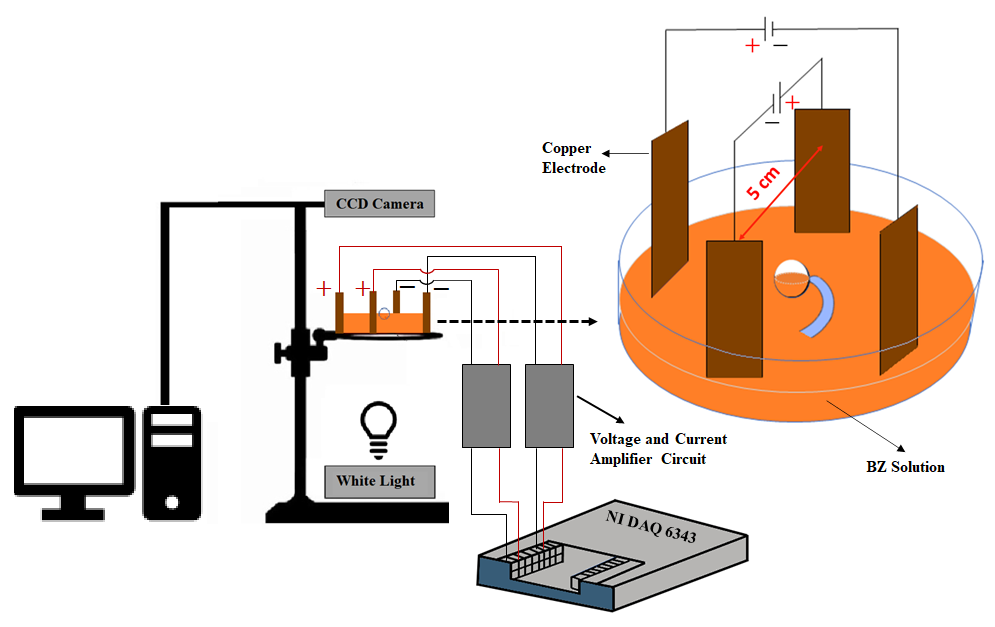
\includegraphics[width=\linewidth]{experiment_setup_01.png}
    \caption{The experimental setup for the polarised filed
      application. Voltage signals from DAQ 6343 are amplified and
      applied to the chemical solution through the cross-arrangement
      of four copper electrodes. }
    \label{fig:ex1}
\end{figure}
To generate voltage signals, we use NI DAQ 6343, also controlled by
LabVIEW software.  We use two copper electrodes for the DC field and a
cross arrangement of four copper electrodes for polarised field
applications. The DAQ can supply a maximum of 20 mA current at the
output. But, the current passing through the solution is more than 20
mA. So, we use electronic circuits designed for current
amplification. An external power supply (LQ 6324T) is used as the
power source for the electronic circuit. The DAQ can generate a signal
with a maximum of $\pm$ 10 V amplitude. Hence the generated signals
should be amplified with appropriate gain. Hence, a non-inverting
amplifier amplifies the output from the DAQ. We require a voltage and
current amplifier circuit for the DC field and the polarised field,
two such circuits with slight modifications.
%\section{Instrumentation}
%\subsection{Experimental methods}
\section{Results and discussion}
We developed two LabVIEW programs to generate both DC and AC
fields. These programs were used to investigate the mechanism of
spiral wave unpinning in the BZ reaction with both DC and polarized
fields.  Our virtual platform is designed to be
intuitive and easy to use, allowing users to adjust the required
parameters, generate voltage signals, monitor wave dynamics, and save
images to a computer for future analysis, all at the same time.
The front panel of the LabVIEW program is shown in Figure
\ref{fig:ex3}. The front panel is
divided into Part I and Part II. Part I is programmed to capture the
images at the desired frame rate.
In our experiment, frame rate is set as 2 fps. 
\begin{figure}[H]
    \centering
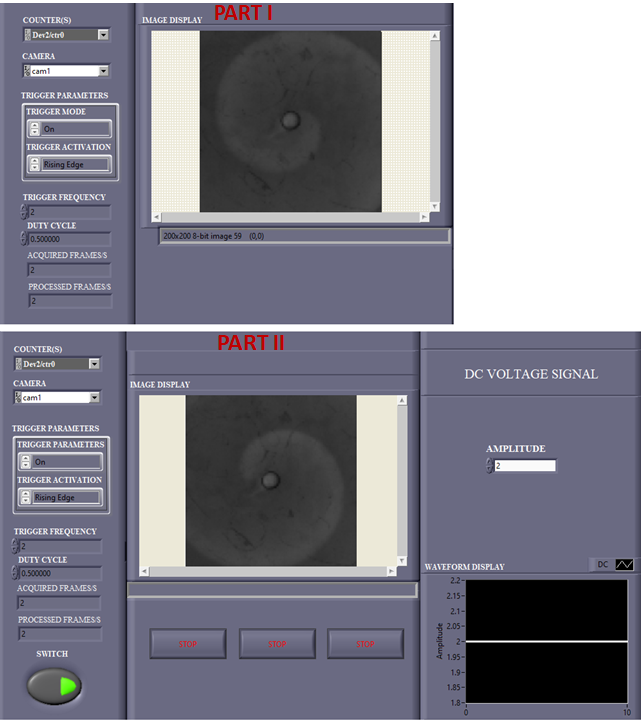
\includegraphics[width=\linewidth]{Dc_frntpnl.png}
    \caption{The front panel of the LabVIEW program for image capture
      and DC voltage generation. Part I of the front panel is for
      image acquisition before the DC voltage generation and part II
      is for image acquisition after the DC voltage generation}
    \label{fig:ex3}
\end{figure}
The front panel contains following icons:
\begin{itemize}
  \item Counters: The image acquisition is controlled using a counter-output trigger
from DAQ 6343. There are four counter-output channels in DAQ 6343. We
use channel counter 0 to trigger the camera.

 \item Camera: The cam1 displays the configured
   camera

   \item Trigger mode: This can be ON or OFF. The program captures the
     images when the trigger mode is ON.  
     \item Trigger activation: The trigger activates
       when the counter signal is at its rising edge or falling edge. We have
       chosen the trigger to activate the camera at its rising edge.
       
     \item trigger frequency: This sets the frame rate of the camera (2 fps).

 \item duty cycle:  the duty cycle of the
   counter trigger.
 \item Acquired frames: the number of images captured per second.
   \item Processed frames:  the number of images
     processed per second.
     \item Switch: allows us to start the DC field application.
     \item Image display: Displays the most recently captured image.
     \item Amplitude: Amplitude of the DC voltage at DAQ ouput can be varied using this numeric control button.
     \item waveform chart: Displays the generated DC voltage at the DAQ output.
\end{itemize}

Part I will stop and part II of the program starts as soon as we press a Boolean switch displayed on the front panel. Part II is programmed to capture the images and generate a DC voltage signal. We use the channel 'analog output 0' (AO 0) of the DAQ to generate the voltage. 
The block diagram corresponding to this front panel is shown in \ref{fig:ex4} (block I) and \ref{fig:ex5} (block II). 
%The block diagram is divided into Block I and Block II. Block I corresponds to part I, and block II corresponds to part II of the front panel. 
Each block is included in a sequence structure that helps to execute the blocks sequentially.
 
The following modules from the LabVIEW library are used:
\begin{itemize}
	\item IMAQdx open camera VI : This VI opens the camera, checking its capabilities, loading the camera configuration file, and creating a distinct reference to the camera. 
	\item IMAQdx property node: We use this node to select trigger parameters displayed on the front panel.
	\item DAQmx create channel (CO Pulse-generation-Frequency) VI : Using this VI, we can choose the Counter channel, frequency, and duty cycle of the trigger.
	\item The DAQmx Start Task VI : Starts the signal generation task.
	\item DAQmx is task done VI: This VI  on the while loop checks whether the signal generation task is completed in each iteration.
	\item The DAQmx configure Grab VI: Configures and starts the grab acquisition.
	\item IMAQdx Grab VI : Captures the images and then passes the images to IMAQ Cast image VI.
	\item IMAQ Cast image VI : convert these RGB frames to grayscale since this reduces the data size.
	\item The IMAQ write file2 VI : Writes the images from IMAQ Caste Image VI to a file in the selected format (png/jpg/bmp/tiff etc.) 
	\item DAQ Assistant Express VI : Generate a DC Voltage at the Analog output 0 (AO 0)
\end{itemize}
%Each image from IMAQ Caste Image VI needs to be written and stored in a folder inside the computer to collect raw image data.  The iteration terminal of the while loop gives the sequential names for images. Each iteration number is converted to a string and concatenated with the file extension and folder path where we need to store images. The String to Path function converts these concatenated strings to a path and is connected to the file path terminal of the 'IMAQ Write file 2 VI'. This connection commands the 'IMAQ Write file 2 VI' to store the images in the mentioned folder with the specified file extension. The While loop helps to run the code continuously. 

%Block II executes as soon as we press the Boolean switch on the front panel. 

%When the ‘switch’ is ON, the case selector terminal of both ‘case structures’ on the block diagram changes to TRUE and corresponding codes execute simultaneously. Code in ‘case structure I’ is for signal generation, and code in case structure II is for image acquisition. "DAQ Assistant Express VI' on the ‘case structure I’ generate a DC Voltage at the Analog output 0 (AO 0). Image acquisition code on 'case structure II' is the same as in block I, but images will be stored in a different folder, and it will stop in the presence of an error or manually pressing a Boolean stop button.

\begin{figure}[H]
	\centering
	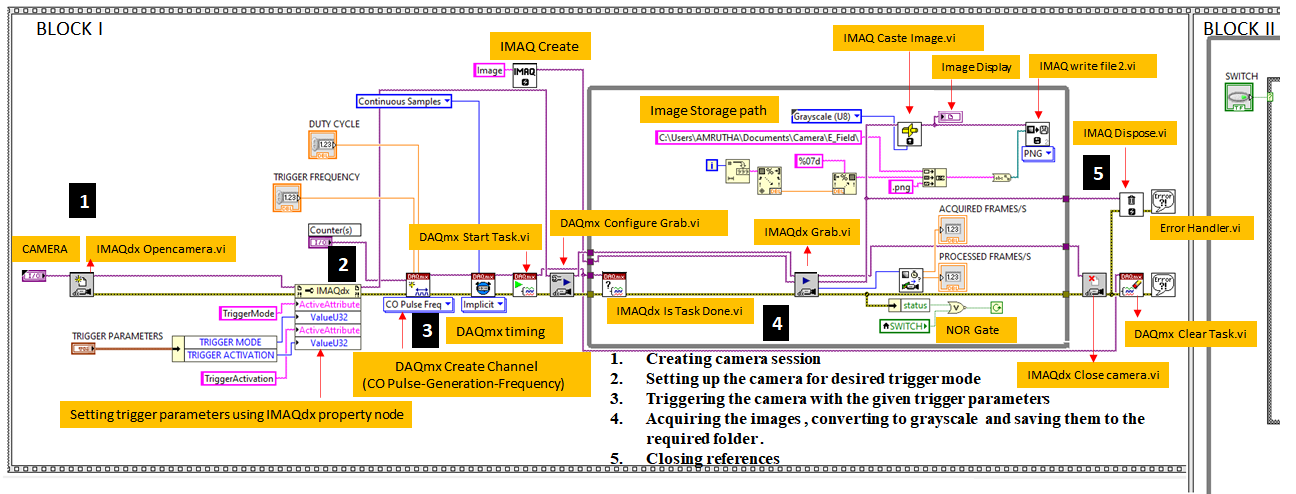
\includegraphics[width=1.3\linewidth,angle=90 ]{Block_1.png}
	\caption{Block diagram of the Image acquisition by triggering the
		camera. Block I captures and saves the images before the DC
		voltage generation.}
	\label{fig:ex4}
\end{figure}

\begin{figure}[H]
	\centering
	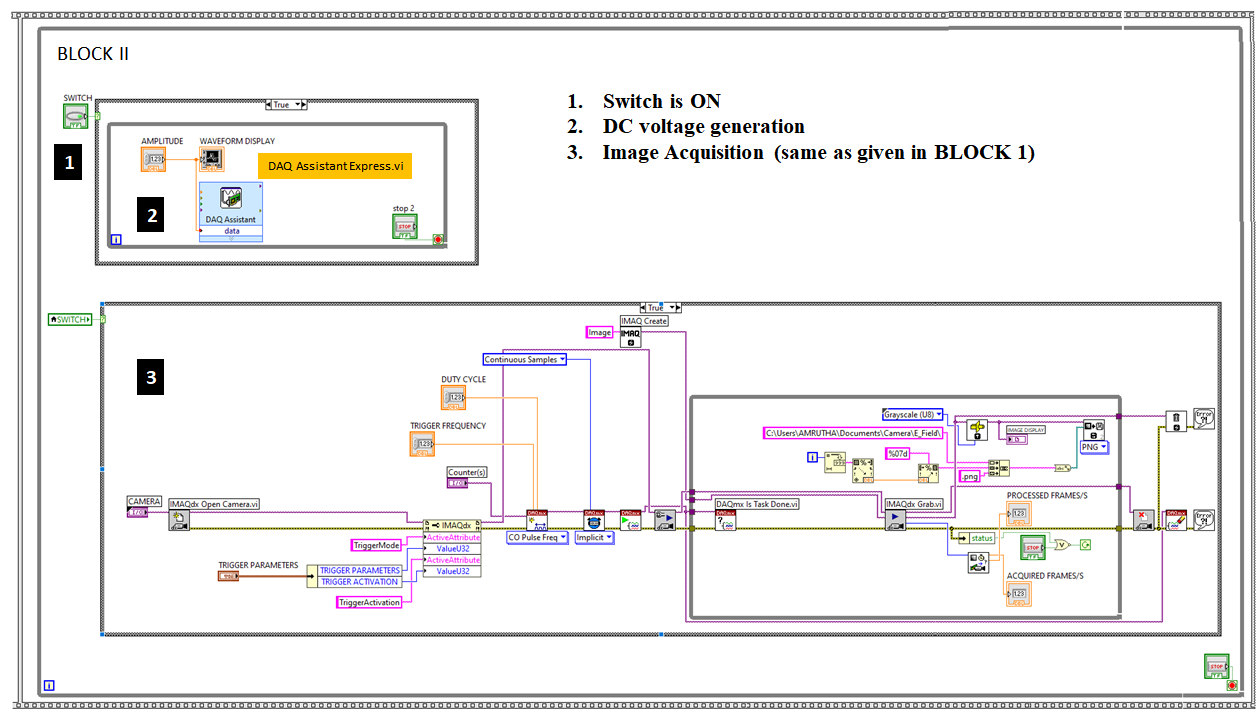
\includegraphics[width=1.3\linewidth,angle=90]{Block_2.png}
	\caption{Block diagram of the image acquisition and DC voltage
		generation. Block II captures and saves the images after DC
		voltage generation.}
	\label{fig:ex5}
\end{figure}


\subsubsection{DC Voltage Signal generation}
\subsubsection{Electronic Circuit for voltage and current amplification}
The NI USB DAQ 6343 generates a DC voltage with user-defined amplitude ($\leq$15V). The output from the non-inverting amplifier is fed to an NPN power transistor (2N6487) capable of handling current (1A) inside the solution. The output from the power transistor is applied to the chemical solution. We can attain a maximum of + 15 V at the output using these electronic setups. The electric field, E, can be varied by using the relation: E= Applied Voltage/distance between electrodes.

\begin{figure}[H]
    \centering
    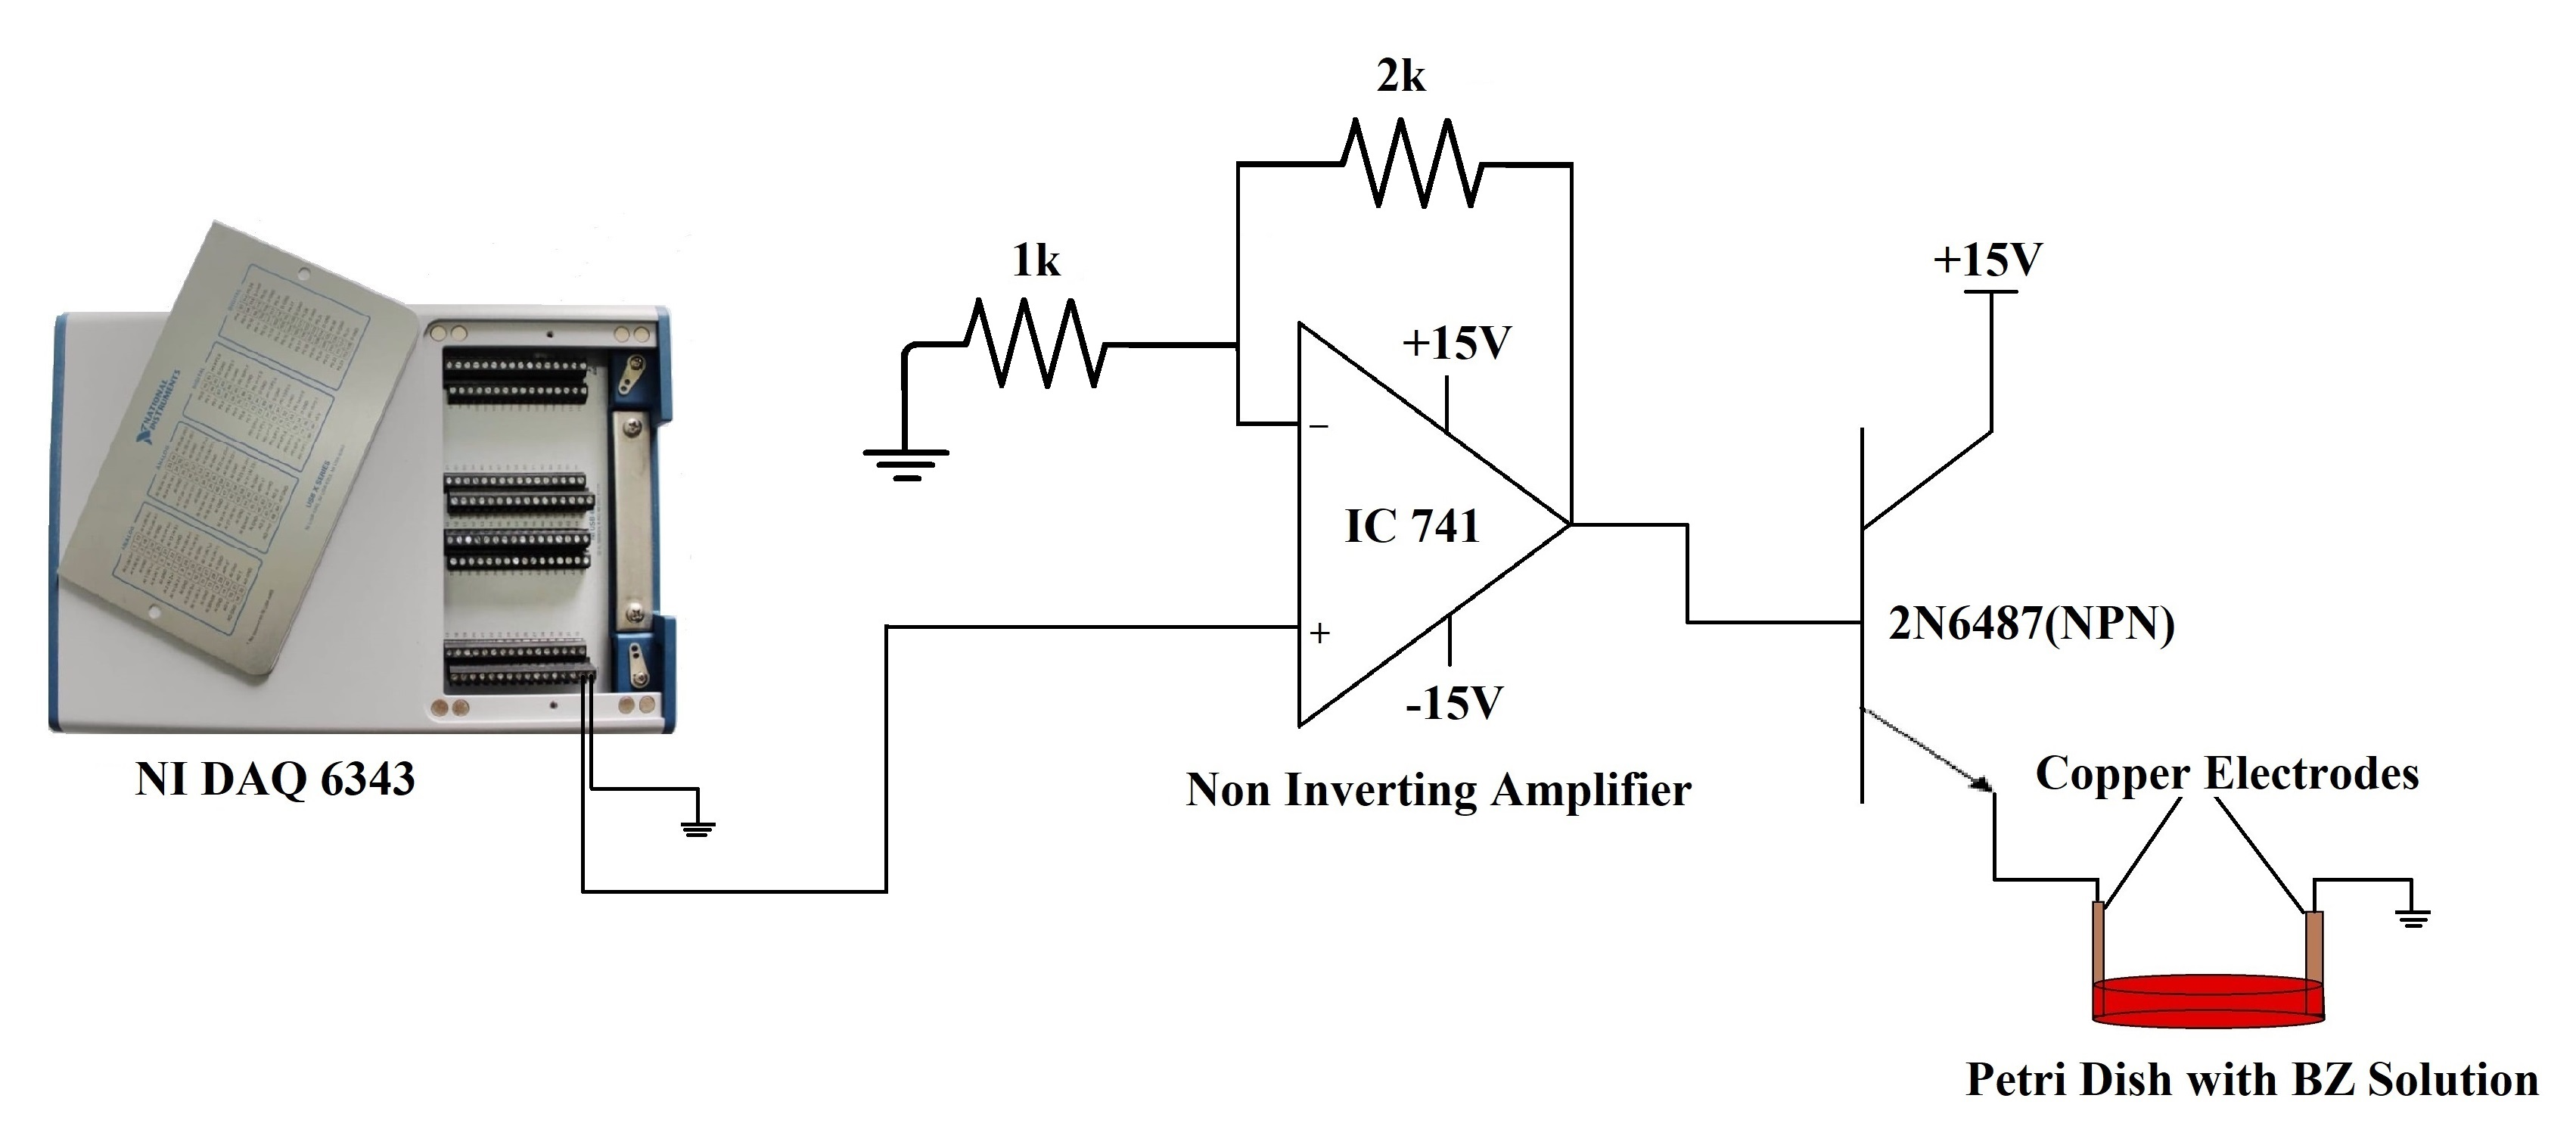
\includegraphics[width=\linewidth]{pulse circuit - Copy.jpg}
    \caption{Shows the voltage and current amplifier circuit for DC
      voltage application in the BZ reaction}
    \label{fig:ex2}
\end{figure}



\subsubsection{Block diagram}
%Figure \ref{fig:ex4} and Figure \ref{fig:ex5} show the block diagram for image acquisition and DC voltage generation. The block diagram isdivided into Block I and Block II. Block I corresponds to part I, and block II corresponds to part II of the front panel. Each block isincluded in a sequence structure that helps execute the blocks sequentially.
 

\subsection{AC Voltage signal Generation}
\subsubsection{Electronic circuit for voltage and current amplification}
To apply a polarised field, we generate two identical AC signals with
a specific phase difference. An electronic circuit is designed with a
push-pull amplifier setup to handle both half cycles of an AC signal.
It includes two matching transistors, one being an NPN-type and the
other a PNP-type. Both power transistors receive the same input
signals equal in magnitude but opposite in phase. This results in one
transistor only amplifying the positive half of the input waveform
cycle while the other amplifies the negative half. The resulting two
halves combine at the output terminal. An error amplifier is also
included to compensate for the input signal fluctuations when we deal
with low-frequency signals. This error amplifier always tries to make
the input and output the same. Identical circuits are required for
each sine wave signal. Signals are applied onto the solution through
copper electrodes as shown in \ref{fig:ex6}.
\begin{figure}[H]
    \centering
    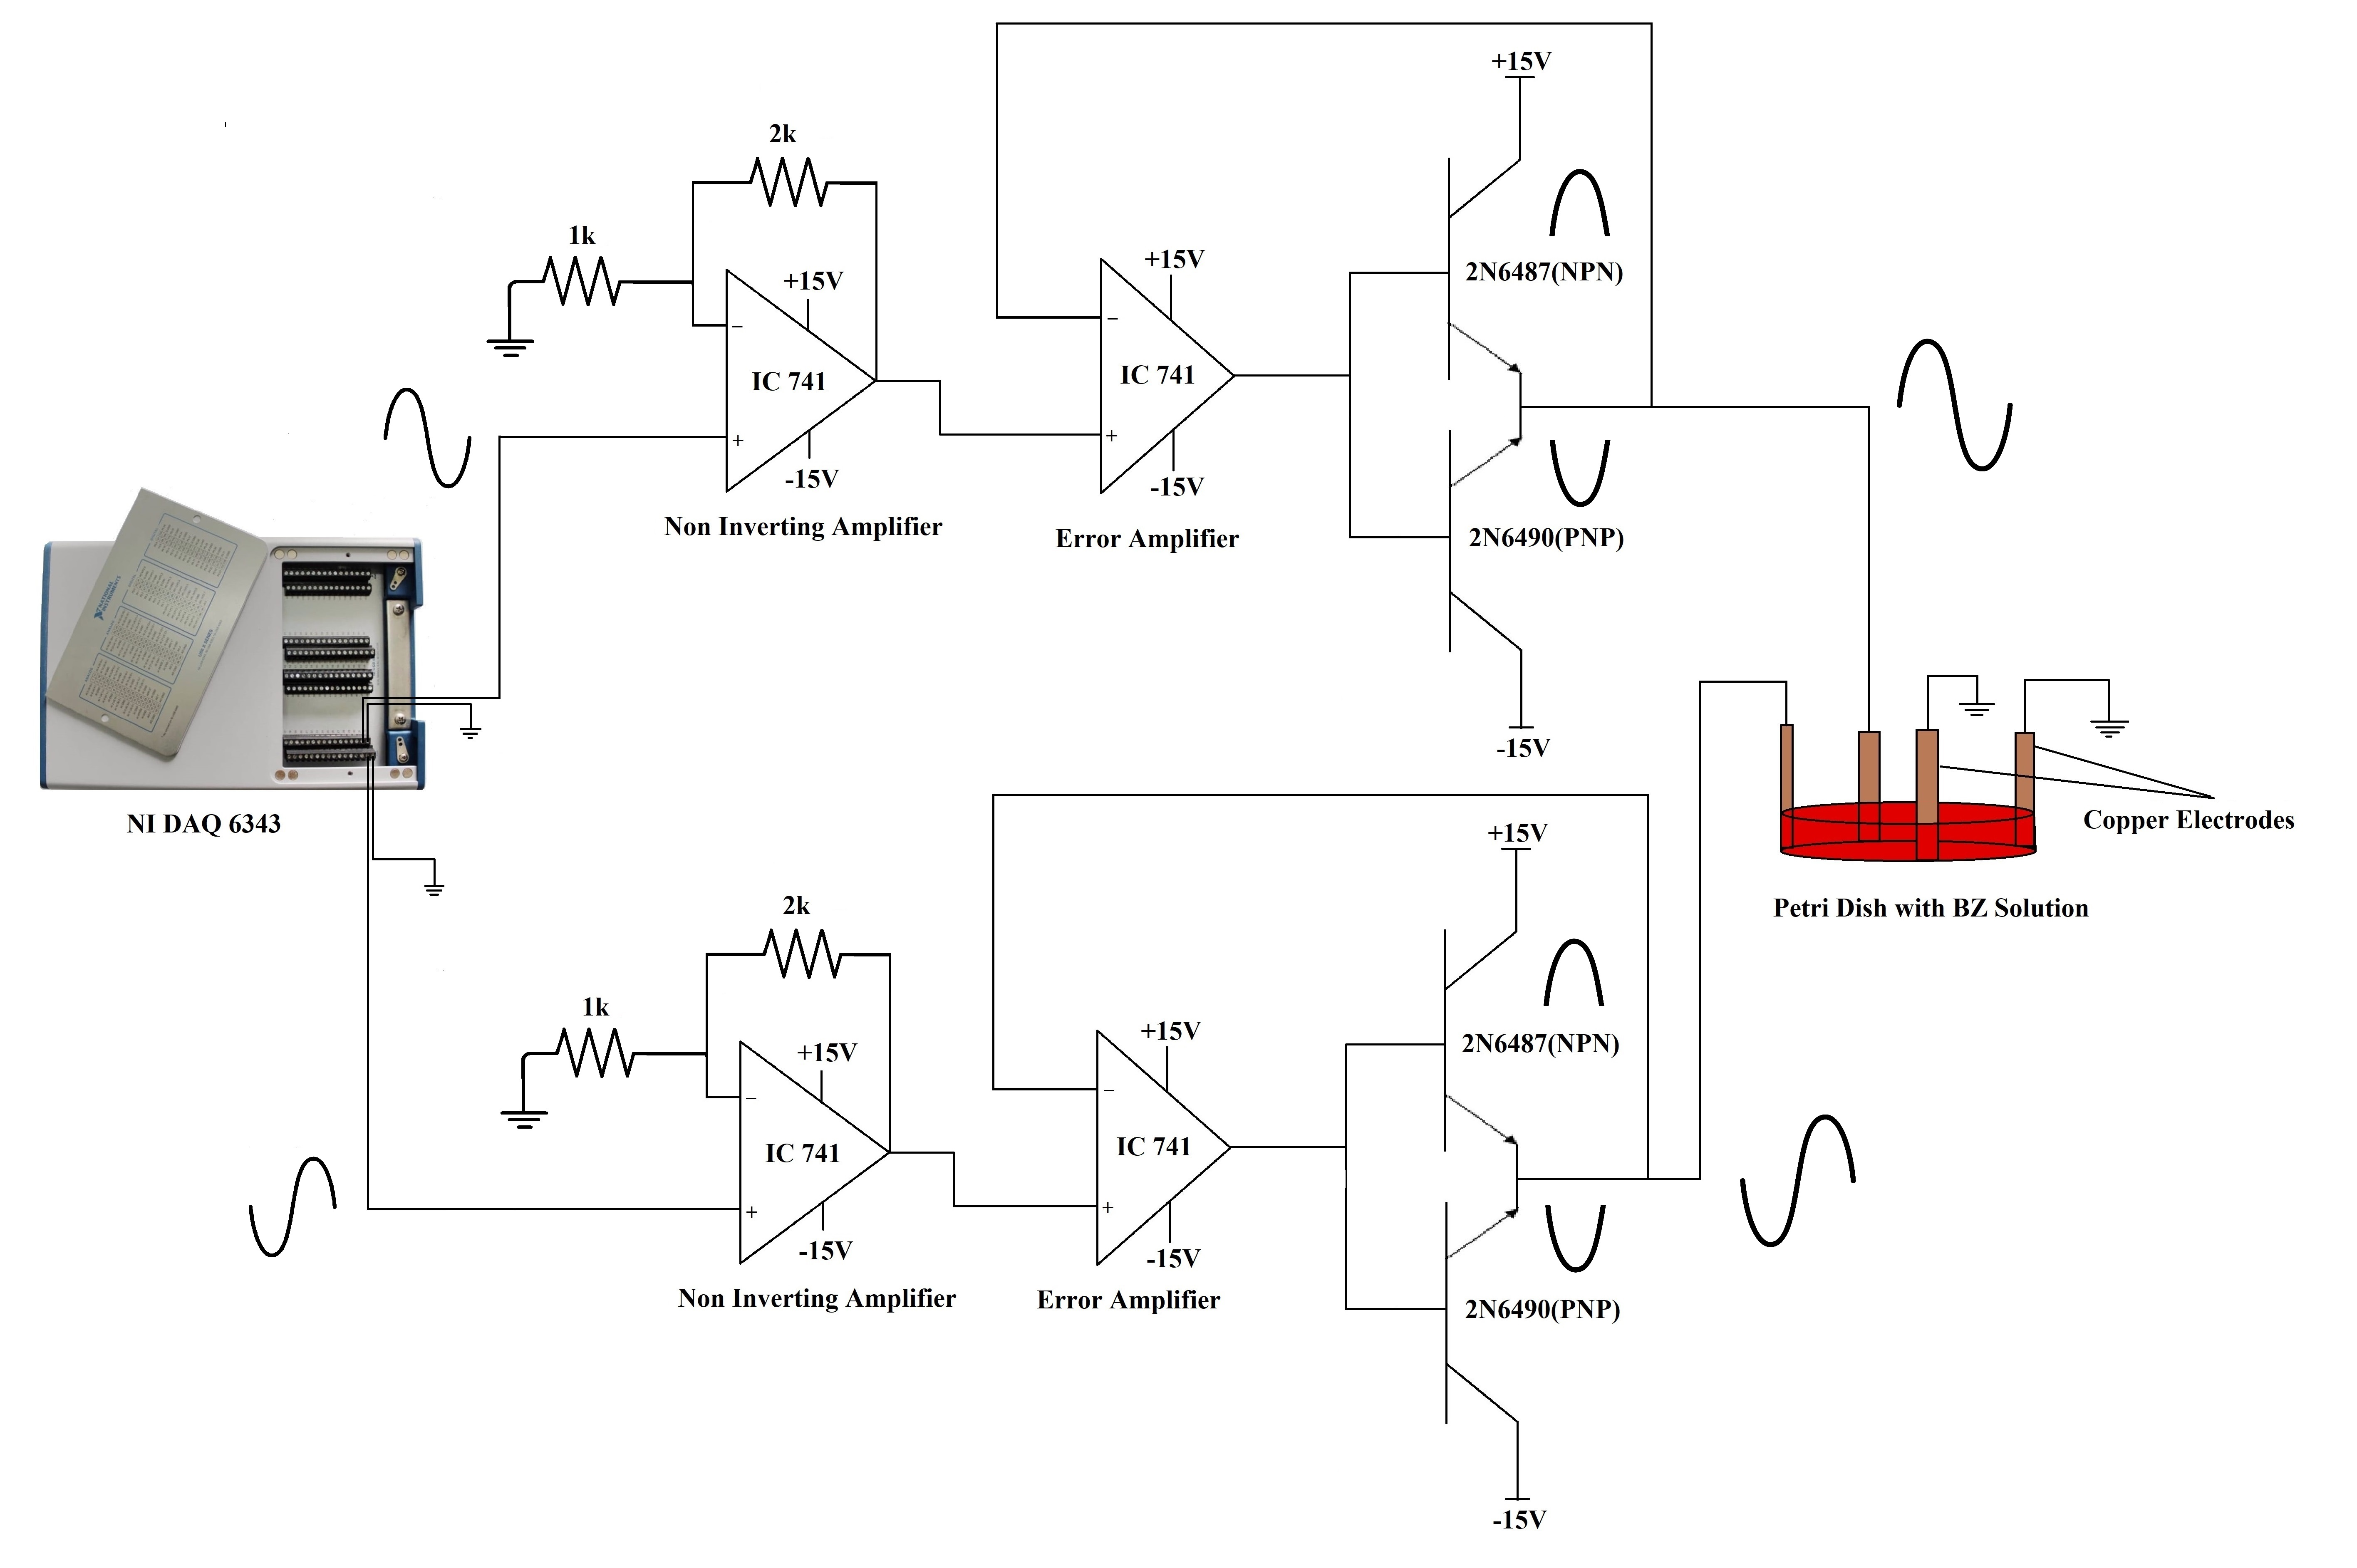
\includegraphics[width=\linewidth]{CPEF - Copy.jpg}
    \caption{Depicts the voltage and current amplifier circuit for a
      pair of AC voltage signal applications in the BZ reaction.}
    \label{fig:ex6}
\end{figure}
%\subsubsection{Front Panel}
The front panel is divided into part I and part II. Part I is
programmed to capture the images with no applied voltage.  Part II is
programmed to capture the images and generate two AC voltage signals
(sine wave or cosine wave). Both parts are the same, as explained
earlier, except for voltage signal generation. 

The front panel contains following new icons:
\begin{itemize}
	\item Physical channels : Describe the analog output channels (AO 0 and AO 1) of the DAQ, which generate two AC voltage signals.
	\item Sampling info: Shows the sampling frequency (Fs) and the number of samples (\#) of the voltage signals.
	\item Amplitude Control Knobs: Used to set the amplitude of the voltage signals.
	\item Frequency : Sets the frequency of the signals.
	\item Phase: Sets the phase of the signals.
	\item The waveform chart: Displays the generated voltage signals at the DAQ output.	
\end{itemize}

\begin{figure}[H]
    \centering
    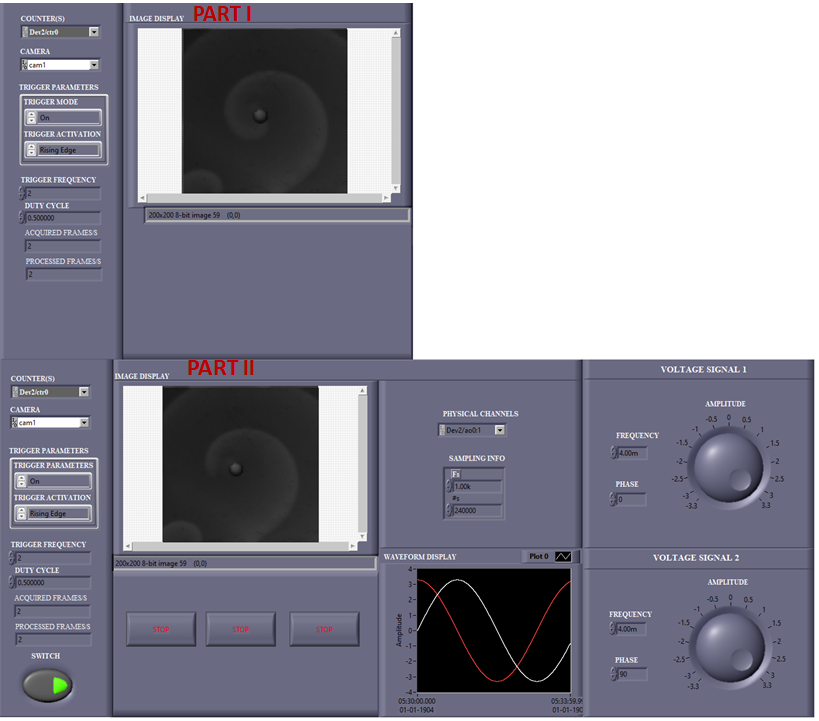
\includegraphics[width=\linewidth]{polarised.png}
    \caption{The front panel of the LabVIEW program for the image
      acquisition and a pair of AC voltage generation. Part I of the
      front panel is for image acquisition before the AC voltage
      generation and part II is for image acquisition after the AC
      voltage generation}
    \label{fig:ex7}
\end{figure}
%\subsubsection{Block Diagram}
The corresponding block diagram is divided into BLOCK I and Block II. Block I is same as we explained as in \ref{fig:ex4}.  \ref{fig:ex9} show the block diagram (BLOCK II) for image acquisition and two AC voltage generation.  Each block is included in a
sequence structure that helps to execute the blocks sequentially. Block II executes as
soon as we press the Boolean switch on the front panel. When the
‘switch’ is ON, the case selector terminal of both ‘case structures’
on the block diagram changes to TRUE and corresponding codes execute
simultaneously. 
Block diagram contains the following modules from the LabVIEW library: 
\begin{itemize}
	\item DAQmx Create Virtual Channel (VI): Creates two different
	output ports (AO 0 \& AO 1) of DAQ Device 6343 to generate two voltage
	signals with user-defined features.
	\item DAQmx timing VI: Sets the source of the sample clock, the rate of the Sample Clock, and the number of samples to generate.
	\item Sine waveform VIs: Creates two sine waves with user-specified amplitude,frequency, phase, and sampling info.
	\item DAQmx Write VI: Writes the waveforms.
	\item DAQmx Start Task VI: Starts the signal generation task.
	\item DAQmx is task done VI: Checks whether the signal generation task is completed in each iteration. 
	\item DAQmx Clear Task VI: clears the task to reduce memory after each iteration.
	\item Error handler VI: displays error messages on the front panel, if any.
\end{itemize}
%Code in ‘case structure I’ is for two AC voltage signal generation and code in ‘case structure II’ is for image acquisition. The image acquisition code on ‘case structure II’ is the same as in block I, but images will be stored in a differentfolder. 
%The sampling info from the ‘sine waveform VI’ is directly fed to ‘DAQmx timing VI'. The waveforms are connected to ‘DAQmx Write VI’ to write them.  This connection commands the DAQ Device to generate signals with the above-mentioned features. Generated signal can be visually observed in the waveformchart displayed on the front panel. The ‘DAQmx Start Task VI’ starts the signal generation task, and ‘DAQmx is task done VI’ on the while loop checks whether the signal generation task is completed in eachiteration.  The ‘DAQmx Clear Task VI’ clears the task to reduce memory after each iteration. The 'while loops' on the block diagram ensure the continuous execution of the code. The ‘Error handler’ displays error messages on the front panel, if any. 

This code is used to achieve different polarised electric fields (linearly polarised,
circularly polarised, and elliptically polarised) if we apply these signals to the chemical solution in four electrode combinations by changing the phase of the signals by keeping the same amplitude and frequency.
\begin{figure}[H]
	\centering
	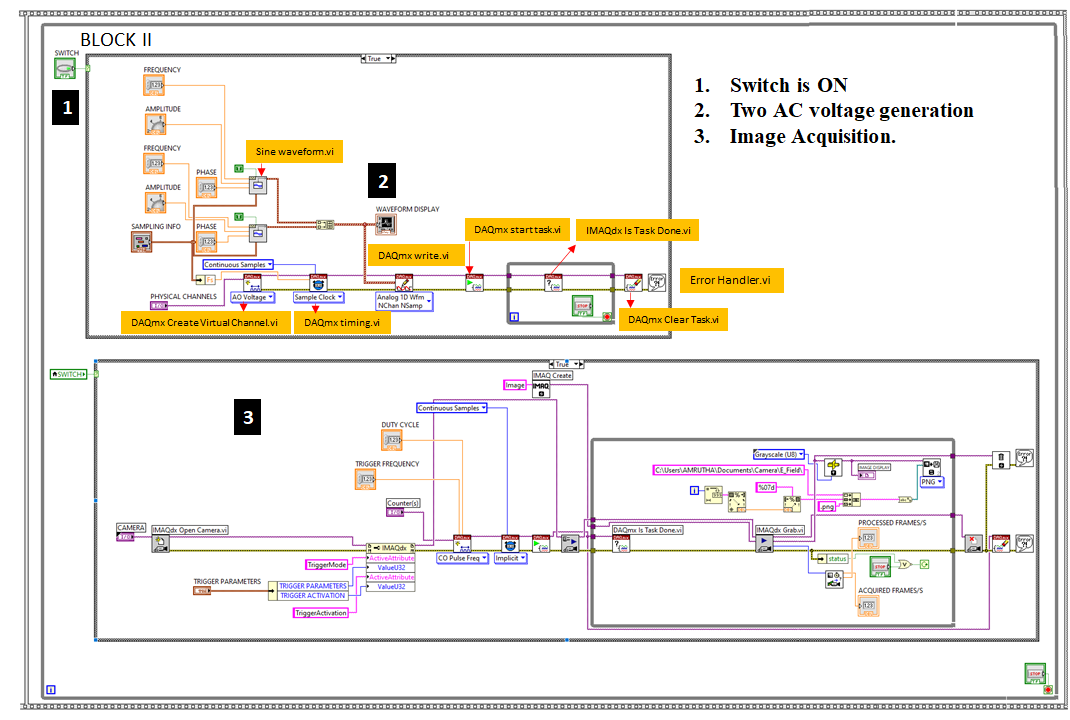
\includegraphics[width=\linewidth, angle=90]{polarised_block_2.png}
	\caption{Block diagram of the image acquisition and a pair of AC voltage generation. Block II
		captures and saves the images after AC voltage generation}
	\label{fig:ex9}
\end{figure}
\section{Conclusions} 
The BZ reaction is a model system for studying chemical and
biological oscillations and provides a platform for exploring the
underlying principles of self-organization and pattern
formation. Spiral and scroll wave unpinning is widely studied in BZ
reaction because of the similarity of the wave dynamics with
biological excitable systems.  The studies in BZ reactions are carried
out using image processing. But due to various factors, imaging the BZ
reaction is challenging. Since the reaction is a non-equilibrium
process and its dynamics change over time, specialized imaging
techniques are required to capture the fast changes and non-stationary
behavior. So, the camera is triggered with counter-output pulses, and
the frequency of the counter signal is used to set the frame rate of
the camera. Additionally, the patterns produced by the BZ reaction can
be difficult to detect since they occur in a semi-transparent
solution. To address this issue, a diffused white LED light source is
placed below the reaction medium, and a blue dichroic filter is
mounted on the camera to enhance imaging. Since the patterns can be
small and occur in three-dimensional space, high spatial-resolution
imaging techniques are required. A CCD camera with a maximum
resolution of 640x480 is used. The user can adjust the required
resolution by changing the image format control option available in NI
Measurements and automation explorer (NI MAX). Furthermore, the BZ
reaction is sensitive to temperature changes, and precise temperature
control is necessary to ensure consistent behavior. Hence, experiments
are performed in an AC room with a controlled ambient temperature.
Unpinning studies use the application of low-voltage electric
fields. Researchers continue to explore new ways to study the BZ
reaction and its excitation wave dynamics using both DC and different
polarised fields. These studies require to control of multiple
instruments simultaneously. Virtual instrumentation allows for
creating of highly accurate, customizable, and easily accessible
instruments that can be used for a wide range of applications. So, we
created two LabVIEW programs to generate DC and AC voltage signals for
the unpinning studies in the BZ reaction. Our programs provide a
user-friendly interface to generate the voltage signals, trigger the
camera, and save the captured images to a computer
simultaneously. With these scripts, we successfully collected the
data, which helped explain the unpinning mechanism in the BZ reaction
in the presence of the DC field and CPEF. One can also modify these
codes and use them to reconstruct scroll waves in the BZ reaction.
%%%%%%%%%%%%%%%%%%%%%%%%%%%%%%%%%%%%%%%%%%%%%%%%%%%%%%%%%%%%
we hope our LabVIEW scripts will be useful for the scientific
community working on BZ reaction or other experiments which involves
image processing and voltage generation by virtual instrumentation.
%%%%%%%%%%%%%%%%%%%%%%%%%%%%%%%%%%%%%%%%%%%%%%%%%%%%%%%%%%%%%%%%%%%%%%%%%%%%%%%%%%%%%%%%%%%%%%%%%%%%%%%%%%%%%%%%%%%%%%%%%%%
%% The "Acknowledgement" section can be given in all manuscript
%% classes.  This should be given within the "acknowledgement"
%% environment, which will make the correct section or running title.
%%%%%%%%%%%%%%%%%%%%%%%%%%%%%%%%%%%%%%%%%%%%%%%%%%%%%%%%%%%%%%%%%%%%%
\begin{acknowledgement}
\end{acknowledgement}

%%%%%%%%%%%%%%%%%%%%%%%%%%%%%%%%%%%%%%%%%%%%%%%%%%%%%%%%%%%%%%%%%%%%%
%% The same is true for Supporting Information, which should use the
%% suppinfo environment.
%%%%%%%%%%%%%%%%%%%%%%%%%%%%%%%%%%%%%%%%%%%%%%%%%%%%%%%%%%%%%%%%%%%%%
\begin{suppinfo}
\end{suppinfo}

%%%%%%%%%%%%%%%%%%%%%%%%%%%%%%%%%%%%%%%%%%%%%%%%%%%%%%%%%%%%%%%%%%%%%
%% The appropriate \bibliography command should be placed here.
%% Notice that the class file automatically sets \bibliographystyle
%% and also names the section correctly.
%%%%%%%%%%%%%%%%%%%%%%%%%%%%%%%%%%%%%%%%%%%%%%%%%%%%%%%%%%%%%%%%%%%%%
\bibliography{achemso-demo}

\end{document}
